\documentclass[aspectratio=169,12pt]{beamer}
\usepackage[utf8]{inputenc}
\usepackage{amsmath, amssymb}
\usepackage{booktabs}
\usepackage{colortbl}
\usepackage{hyperref}
\usepackage{makecell}
\usepackage{ragged2e}
\usepackage{tikz}
\usetikzlibrary{arrows.meta, positioning, shapes.geometric, calc, tikzmark, shapes.misc, fit, decorations.pathreplacing}
\usepackage{tcolorbox}
\usepackage{array}
\usepackage{listings}
\usetheme{Madrid}

% Custom colors
\definecolor{correctgreen}{RGB}{0,150,0}
\definecolor{incorrectred}{RGB}{200,0,0}
\definecolor{counterblue}{RGB}{70,130,255}
\definecolor{highlightyellow}{RGB}{255,230,100}
\definecolor{lightblue}{RGB}{200,230,250}
\definecolor{darkblue}{RGB}{0,100,200}

% Code listing settings
\lstset{
    basicstyle=\ttfamily\small,
    keywordstyle=\color{blue},
    commentstyle=\color{gray},
    numbers=left,
    numberstyle=\tiny\color{gray},
    frame=single,
    breaklines=true
}

\title{Out-of-Order Execution (OOOE)}
\subtitle{Computer Architecture - Example Problem}
\author{Course 234267}
\date{}

\begin{document}

\begin{frame}
\titlepage
\end{frame}

\begin{frame}{Outline}
\tableofcontents
\end{frame}

\section{System Specification}

\begin{frame}{OOOE System Specification}
\begin{block}{System Capabilities}
Our Out-of-Order Execution system has the following characteristics:
\end{block}

\begin{itemize}
    \item \textbf{Fetch Stage:} 2 instructions per clock cycle
    \item \textbf{Decode Stage:} 2 instructions per clock cycle  
    \item \textbf{Integer ALU:} 2 operations per clock cycle
    \begin{itemize}
        \item Each ALU operation takes only 1 cycle
    \end{itemize}
    \item \textbf{Load/Store Operations:} 5 clock cycles
    \begin{itemize}
        \item Operations are \textbf{not} pipelined
        \item Take 5 cycles to complete
    \end{itemize}
\end{itemize}
\end{frame}

\begin{frame}{System Components}
\begin{columns}
\column{0.5\textwidth}
\begin{block}{Hardware Structures}
\begin{itemize}
    \item \textbf{RS} - Reservation Station (unbounded)
    \item \textbf{MOB} - Memory Order Buffer (unbounded)
    \item \textbf{ROB} - Reorder Buffer (unbounded)
    \item \textbf{RAT} - Register Alias Table
    \item \textbf{IDQ} - Instruction Decode Queue
\end{itemize}
\end{block}

\column{0.5\textwidth}
\begin{block}{Additional Features}
\begin{itemize}
    \item Full bypassing support between all stages
    \item Ideal branch prediction (never mispredicts)
    \item All queues are effectively unlimited in size
\end{itemize}
\end{block}
\end{columns}
\end{frame}

\section{Example Program}

\begin{frame}[fragile]{Original Program - High Level}
\begin{columns}
\column{0.5\textwidth}
\begin{lstlisting}[language=C]
R0 = 0
R1 = 0
L1: R4 = 20
    R5 = load 100(R4)
    R3 = R2 + 2
    R5 = R3 + 2
    R6 = 6
    R7 = R5
    R8 = 8
    R9 = 9
    R1 = R1 + 1
    IF (R1 < 100) goto L1
L2: R4 = 23
\end{lstlisting}

\column{0.5\textwidth}
\begin{block}{Key Points}
\begin{itemize}
    \item Loop executes 100 times
    \item Contains mix of ALU and memory operations
    \item Load instruction creates potential dependencies
    \item Several register assignments in loop body
\end{itemize}
\end{block}
\end{columns}
\end{frame}

\begin{frame}[fragile]{Assembly Translation}
\begin{lstlisting}[basicstyle=\ttfamily\footnotesize]
    ADDI R10, R0, 100      ; Set loop counter limit
    SUB  R1, R1, R1        ; Initialize R1 = 0
L1: ADDI R4, R0, 20        ; R4 = 20
    LW   R5, 100(R4)       ; Load from memory[R4+100]
    ADDI R3, R2, 2         ; R3 = R2 + 2
    ADDI R5, R3, 2         ; R5 = R3 + 2
    ADDI R6, R0, 6         ; R6 = 6
    ADD  R7, R5, R0        ; R7 = R5
    ADDI R8, R0, 8         ; R8 = 8
    ADDI R9, R0, 9         ; R9 = 9
    ADDI R1, R1, 1         ; Increment loop counter
    BNE  R1, R10, L1       ; Branch if R1 != 100
L2: ADDI R4, R0, 23        ; R4 = 23
\end{lstlisting}
\end{frame}

\section{Execution Analysis}

\begin{frame}{OOO Execution Pipeline}
\begin{figure}
\centering
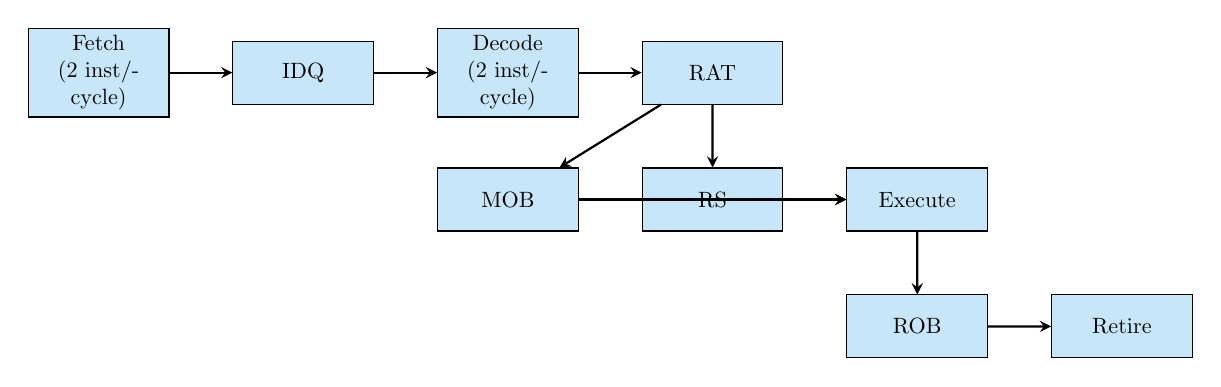
\begin{tikzpicture}[scale=0.8, transform shape]
    % Define styles
    \tikzstyle{block} = [rectangle, draw, fill=lightblue, 
                          text width=2cm, text centered, 
                          minimum height=1cm]
    \tikzstyle{arrow} = [thick,->,>=stealth]
    
    % Create blocks
    \node[block] (fetch) {Fetch\\(2 inst/cycle)};
    \node[block, right=of fetch] (idq) {IDQ};
    \node[block, right=of idq] (decode) {Decode\\(2 inst/cycle)};
    \node[block, right=of decode] (rat) {RAT};
    
    \node[block, below=of rat] (rs) {RS};
    \node[block, right=of rs] (exec) {Execute};
    \node[block, left=of rs] (mob) {MOB};
    
    \node[block, below=of exec] (rob) {ROB};
    \node[block, right=of rob] (retire) {Retire};
    
    % Draw arrows
    \draw[arrow] (fetch) -- (idq);
    \draw[arrow] (idq) -- (decode);
    \draw[arrow] (decode) -- (rat);
    \draw[arrow] (rat) -- (rs);
    \draw[arrow] (rat) -- (mob);
    \draw[arrow] (rs) -- (exec);
    \draw[arrow] (mob) -- (exec);
    \draw[arrow] (exec) -- (rob);
    \draw[arrow] (rob) -- (retire);
\end{tikzpicture}
\end{figure}
\end{frame}

\begin{frame}{Execution Timeline - Second Loop Iteration}
\begin{block}{Question}
Show the system state when completing the fetch of instruction L1 for the second time.
\end{block}

\begin{itemize}
    \item Track instruction flow through pipeline stages
    \item Monitor reservation stations and ROB entries
    \item Identify dependencies and hazards
    \item Calculate execution cycles
\end{itemize}
\end{frame}

\begin{frame}{Key Execution Cycles}
\begin{table}
\centering
\begin{tabular}{|c|l|l|}
\hline
\textbf{Cycle} & \textbf{Operations} & \textbf{Notes} \\
\hline
1 & Fetch first 2 instructions & ADDI R10, SUB R1 \\
\hline
2 & Decode, Fetch next 2 & ADDI R4, LW R5 \\
\hline
3 & Issue to RS/MOB & Load enters MOB \\
\hline
4-6 & Execute ALU ops & Load in progress \\
\hline
7 & Second iteration fetch & RAW dependency \\
\hline
\end{tabular}
\end{table}

\begin{alertblock}{Critical Path}
The load instruction creates a 5-cycle latency that affects dependent instructions.
\end{alertblock}
\end{frame}

\section{Performance Analysis}

\begin{frame}{CPI Calculation}
\begin{block}{Performance Metrics}
\begin{itemize}
    \item Loop contains 10 instructions
    \item Executes 100 iterations
    \item From first LW fetch (cycle 2) to second LW fetch (cycle 7): 5 cycles
    \item No delays from memory reads after first iteration
    \item Structural hazard doesn't cause delays (only 1 instruction in EXE at times)
\end{itemize}
\end{block}

\begin{tcolorbox}[colback=highlightyellow,colframe=darkblue]
\textbf{Result:} CPI $\approx$ 0.5
\begin{itemize}
    \item System can sustain 2 instructions per cycle
    \item OOO execution hides latencies effectively
\end{itemize}
\end{tcolorbox}
\end{frame}

\section{Compiler Optimization}

\begin{frame}[fragile]{Compiler Optimization}
\begin{columns}
\column{0.45\textwidth}
\textbf{Original Code:}
\begin{lstlisting}[basicstyle=\ttfamily\tiny]
R0 = 0
R1 = 0
L1: R4 = 20
    R5 = load 100(R4)
    R3 = R2+2
    R5 = R3 + 2
    R6 = 6
    R7 = R5
    R8 = 8
    R9 = 9
    R1 = R1 + 1
    IF (R1 < 100) goto L1
L2: R4 = 23
\end{lstlisting}

\column{0.45\textwidth}
\textbf{Optimized Code:}
\begin{lstlisting}[basicstyle=\ttfamily\tiny]
R0 = 0
R1 = 0
R4 = 20
R6 = 6
R8 = 8
R9 = 9
L1: R5 = load 100(R4)
    R3 = R2+2
    R5 = R3 + 2
    R1 = R1 + 1
    IF (R1 < 100) goto L1
R7 = R5
L2: R4 = 23
\end{lstlisting}
\end{columns}

\begin{block}{Optimization: Loop Invariant Code Motion}
Move constant assignments outside the loop!
\end{block}
\end{frame}

\begin{frame}{Impact of Optimization}
\begin{block}{Analysis}
\begin{itemize}
    \item \textbf{Before:} 10 instructions in loop
    \item \textbf{After:} 5 instructions in loop
    \item \textbf{BUT:} Load operation still takes 5 cycles
    \item Load operations cannot execute in parallel
\end{itemize}
\end{block}

\begin{alertblock}{Performance Result}
\begin{itemize}
    \item CPI increases by factor of $\approx 2$
    \item IC (Instruction Count) decreases by factor of $\approx 2$
    \item \textbf{Total execution time: No significant change!}
\end{itemize}
\end{alertblock}

\begin{block}{Key Insight}
Runtime = IC × CPI × Clock Period
\end{block}
\end{frame}

\section{Hardware Improvements}

\begin{frame}{Proposed Hardware Enhancement}
\begin{block}{Question}
Adding a third ALU unit - does it improve performance?
\end{block}

\begin{columns}
\column{0.5\textwidth}
\begin{block}{Answer: No}
\begin{itemize}
    \item Structural hazard was not the bottleneck
    \item Load latency dominates execution time
    \item Additional ALU remains unused
\end{itemize}
\end{block}

\column{0.5\textwidth}
\begin{block}{Better Improvements}
\begin{itemize}
    \item Faster load execution (< 5 cycles)
    \item Parallel load execution units
    \item Better memory hierarchy
    \item Prefetching mechanisms
\end{itemize}
\end{block}
\end{columns}
\end{frame}

\section{Conclusions}

\begin{frame}{Key Takeaways}
\begin{enumerate}
    \item \textbf{OOO Execution Benefits:}
    \begin{itemize}
        \item Hides latencies through parallel execution
        \item Achieves CPI < 1 with proper resources
    \end{itemize}
    
    \item \textbf{Memory Operations are Critical:}
    \begin{itemize}
        \item 5-cycle load latency creates bottlenecks
        \item Cannot be easily hidden even with OOO
    \end{itemize}
    
    \item \textbf{Compiler Optimizations:}
    \begin{itemize}
        \item May reduce instruction count
        \item Don't always improve performance
        \item Must consider hardware constraints
    \end{itemize}
    
    \item \textbf{Hardware Improvements:}
    \begin{itemize}
        \item Must target actual bottlenecks
        \item Memory subsystem often more critical than ALUs
    \end{itemize}
\end{enumerate}
\end{frame}

\begin{frame}{Thank You!}
\centering
\Large Questions?

\vspace{1cm}

\normalsize
Computer Architecture\\
Course 234267
\end{frame}




\end{document}